\chapter{METHODOLOGY}
\section{System Design}

The purpose of the helmet detection system is to track helmet use from CCTV footage on a college campus. Three primary phases of the system comprise data preparation, model training and system implementation. The first step involves converting campus CCTV video footage into image frames, which are subsequently labelled with helmet and unhelmeted head information using Roboflow. A customised YOLOv8 object detection model that is tuned for real-time performance is trained using the annotated dataset. After training, the model is incorporated into a real-time system that recognises and categorises heads and helmets by processing incoming video frames. In order to provide real-time statistics that facilitate safety compliance monitoring, a counting mechanism is integrated to monitor the quantity of helmets and heads seen within a designated area of interest.


\begin{figure}[H] % Optional: [H] requires \usepackage{float}
	
	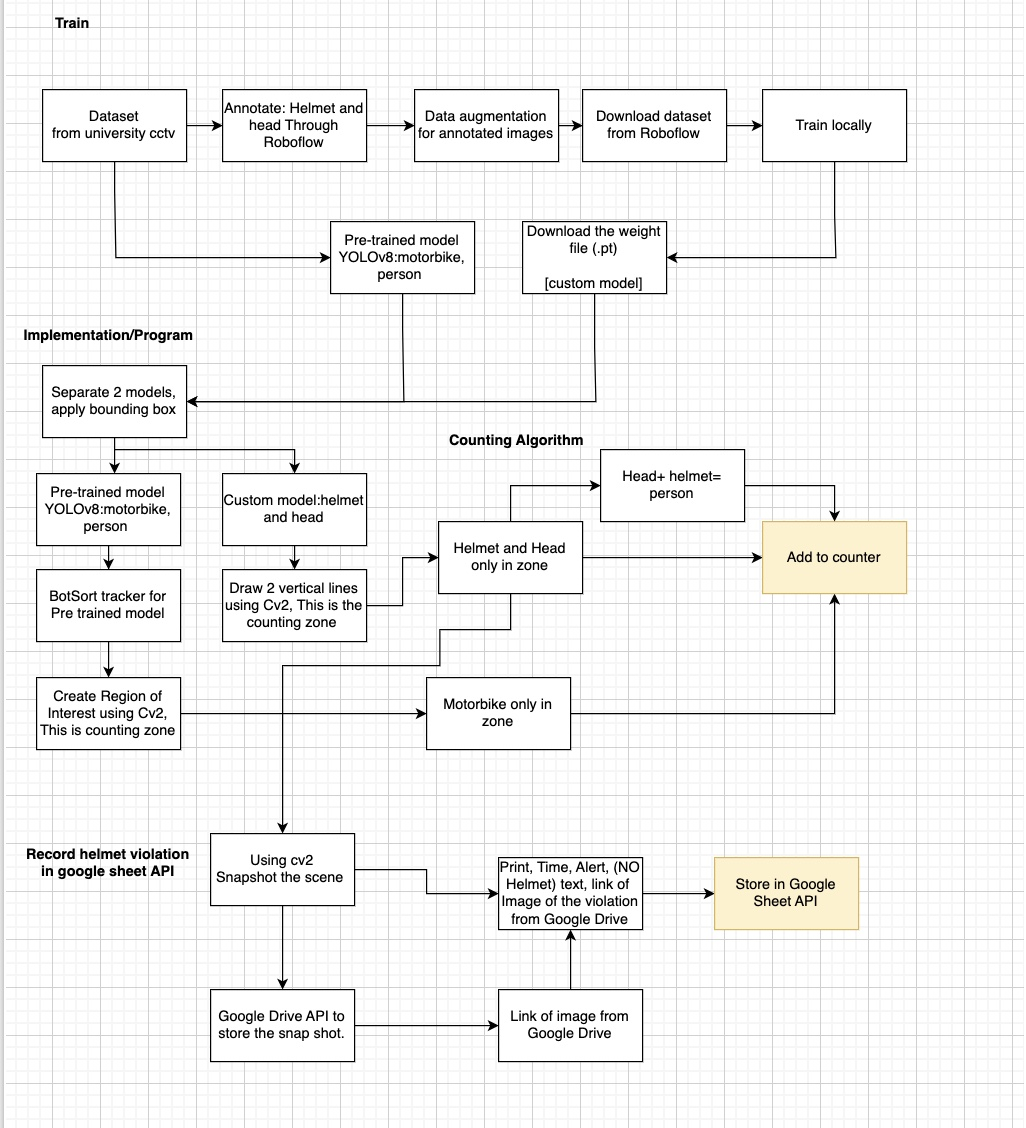
\includegraphics[width=1\textwidth]{flowchart.jpg}
	\vspace{0.5em}
	\centering
	\noindent\textbf{Figure 3.1} \\
	\caption*{} % Optional: if you want a caption, otherwise keep empty
	
	
\end{figure}

The flowchart in the figure 3.1 illustrates the overall workflow of the system. First, the dataset is obtained from the footages of a cctv camera of Mahidol university. The video footages are split into 3 frames per second using Roboflow. Then annotate each frames splited, the annoated items are helmet and head, then using data augmentations from Roboflow. Then we can downlaod the datasets. Finally, using dataset downloaded we can train locally through data.yaml, the data augmentations details are to be specified in Chapter 3. After the training the weights of the trained model are obtained in a .pt file, the file is the model that will be used in the system in conjunction with the pre-trained model from YOLOv8. The Implementation phase is to apply the custom trained model called best\_17, work with the video stream input. The bounding box and region of interest seen in figure 3.2.made from cv2. 

	\begin{center}
	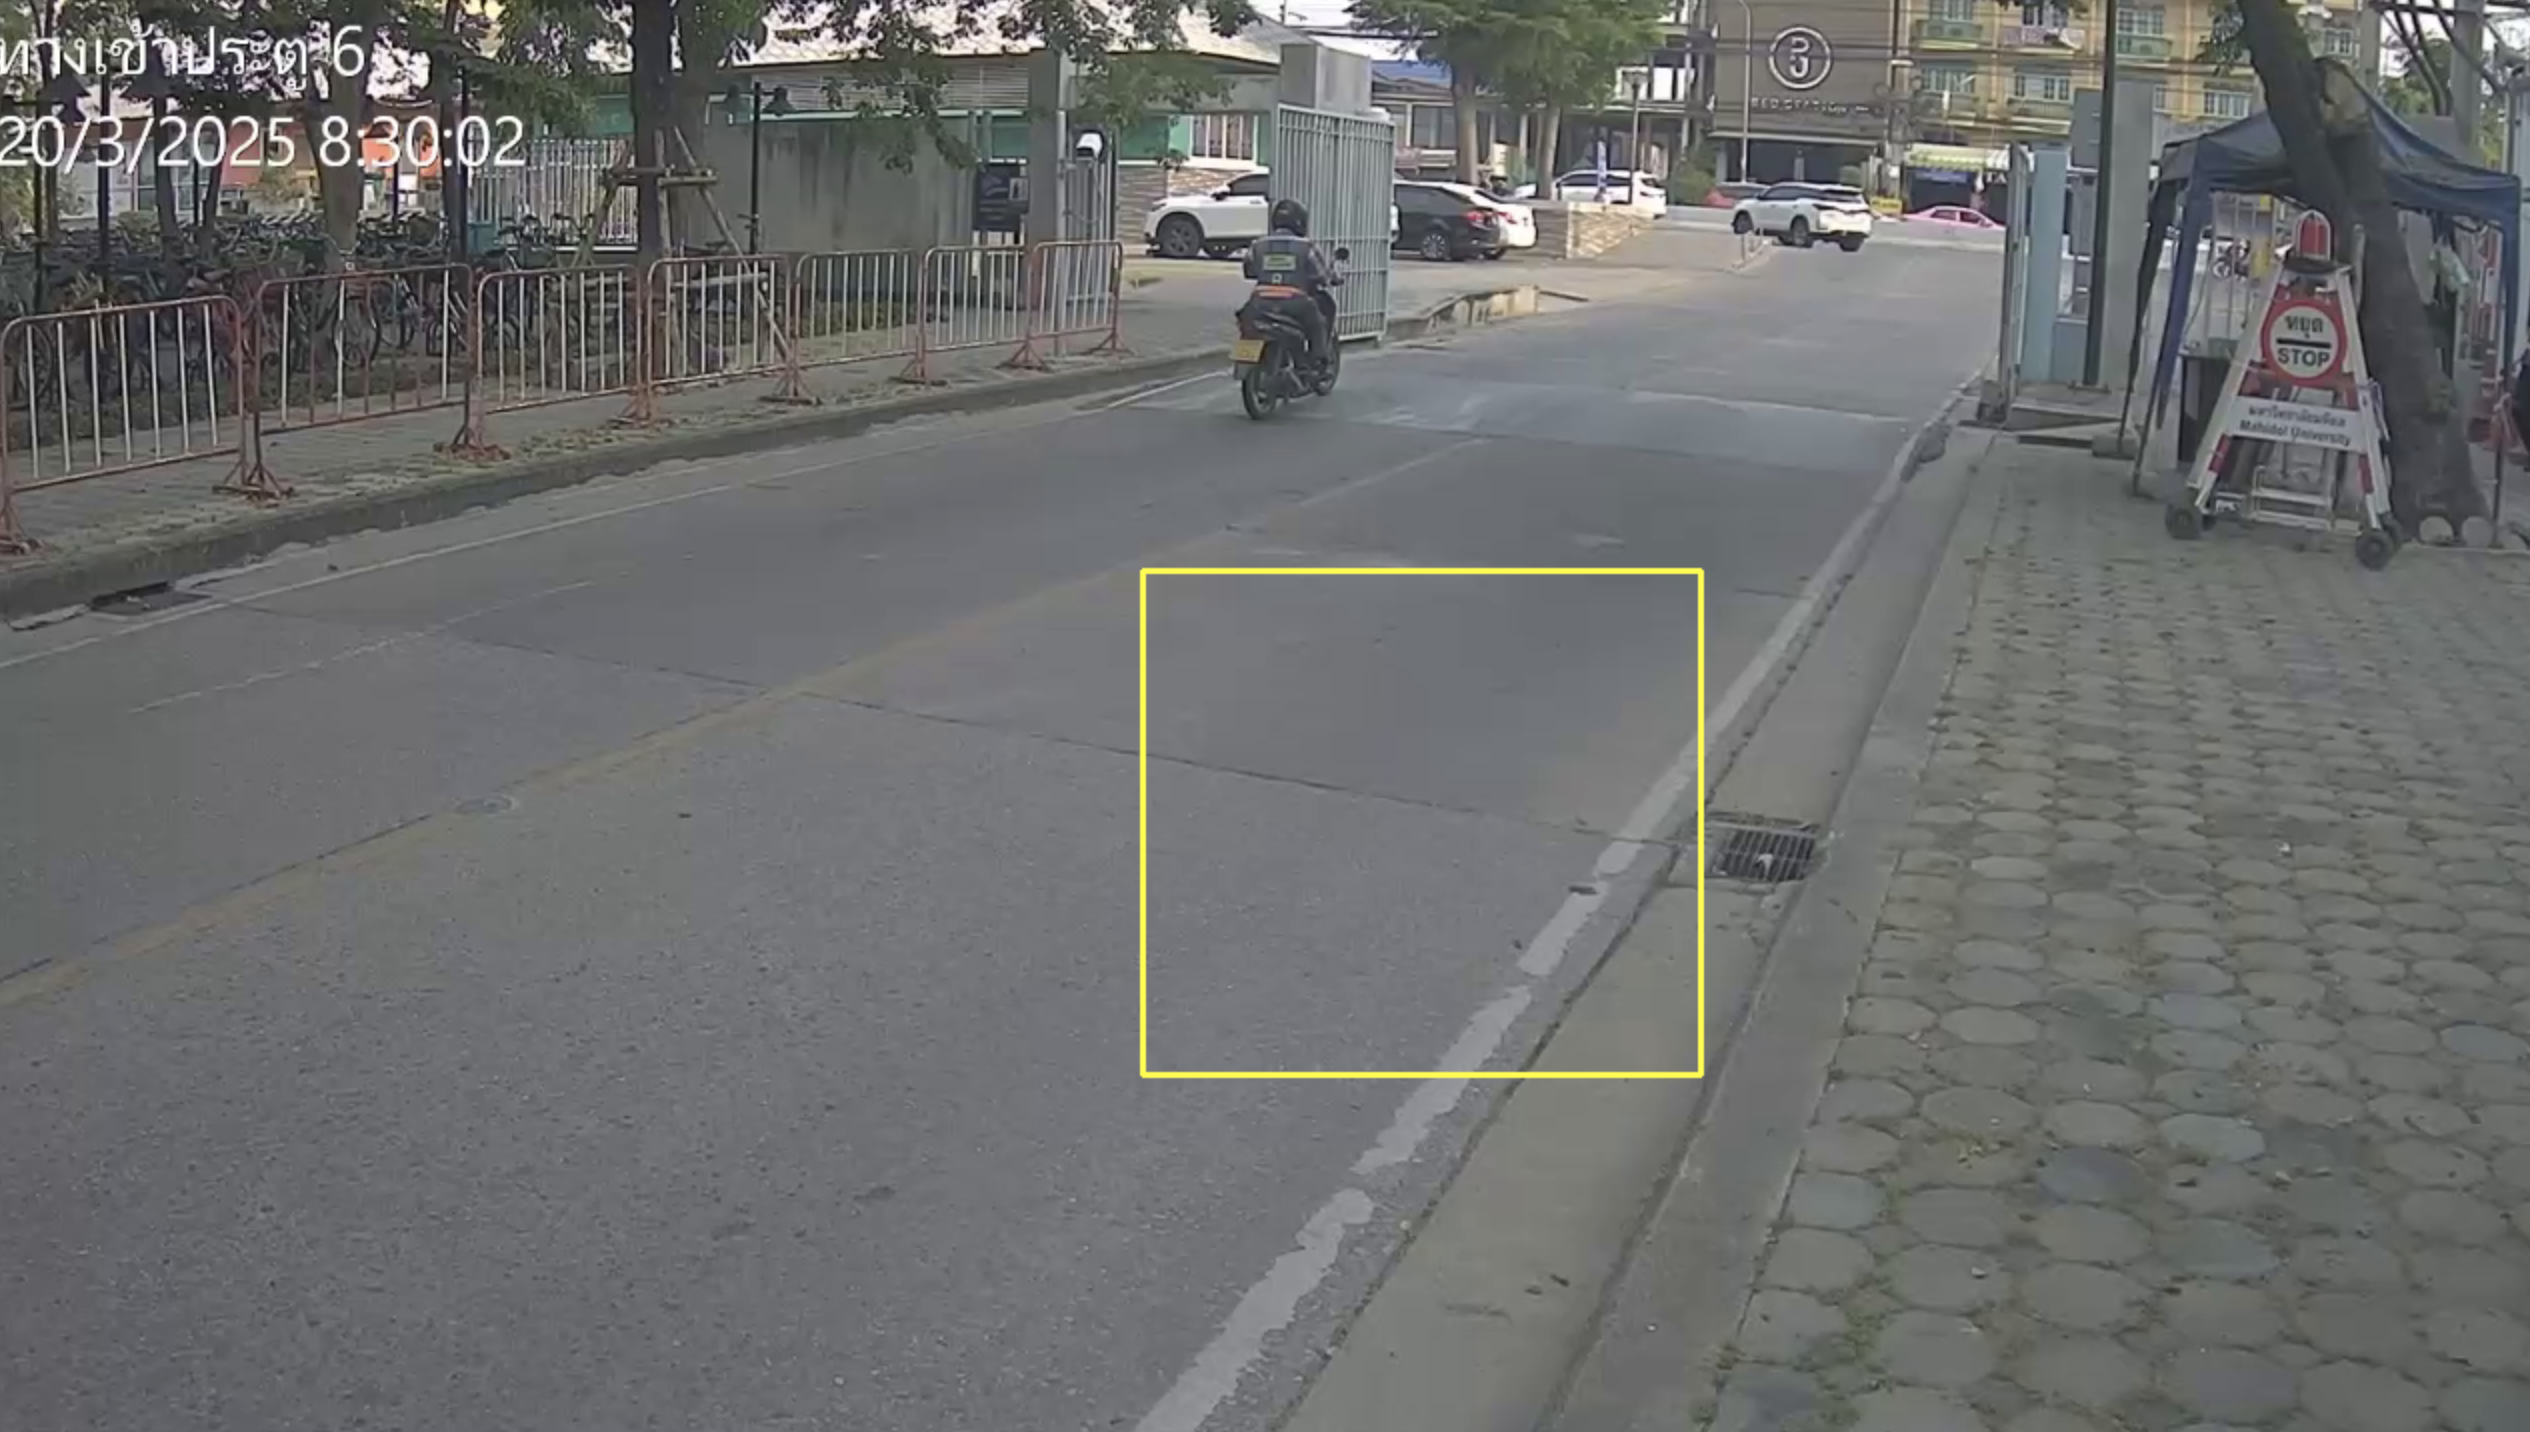
\includegraphics[width=0.5\textwidth]{ROI.png}
	
	\vspace{0.5em}
	\textbf{Figure 3.2: Dataset Image}
`\end{center}

Using these zone we speparate the counting zone for helmet, head, and another zone to count person and helmet. As for the person we decided to count the head and the helmet to total to person as there are issues about the camera angel limiting the accuracy of the person detection. 

After implementing the program with the model, we use cv2 to take snapshot of the frame as when helmet violation occur. The system links and uses Google API, to store the detection evidence of the scenario. The Google Sheet API will append new rows each time a head detection occur.  The image are visible, and stored by Google Drive API, to check the instances where it happens.

\section{Data}
Dataset: videos of the entrance which contain motorcycle coming in and out the campus, collected from local sources which is gate six Mahidol University CCTV camera. The videos are split into frames using Roboflow and then each frame are use for annotations.
\newline
\newline
Annotations: Create two classes. first class containing the bouding box of helmet user only and the second class containing head(which is non-helmet user.)
\newline
Preprocessing: Includes resizing images to 640x640 pixels, normalizing pixel values, and applying augmentations (e.g., rotation, scaling, and brightness adjustments).

\newpage
\section{Custom Model}
\textbf{YOLOv8 Architecture:}
YOLOv8 (You Only Look Once version 8), developed by Ultralytics, is known for its streamlined architecture and improved detection performance over its predecessors (e.g., YOLOv5, YOLOv7), particularly in low-light or occluded environments—conditions often encountered in real-world surveillance footage. The YOLOv8 architecture is used for this project due to its state-of-the-art performance in object detection, offering a balance between real-time inference speed and high accuracy. Specifically for this project, YOLOv8 is a tool that is important for training and differentiating helmet and head classes easily. Additionally YOLOv8 is easier to set up and supported by developers and communities in a larger scale than other YOLO versions.

Despite the availability of newer object detection models such as YOLO-NAS or YOLOv9, YOLOv8 remains a highly reliable and widely supported choice. In this project, YOLOv8 was used to create a custom-trained model that focuses on five specific object classes: motorcycles, helmets, crosswalks, pedestrians, and lanes. However, the two most critical objects for our safety analysis—helmet and head—were prioritized in both annotation and evaluation.


To obtain the custom model for "head", and "helmet" detection we must first upload the datasets into Roboflow website in figure 3.1. Roboflow will allow users to specifically annotate desired classes, which after annotating said datasets, we can download directly from Roboflow the annotated datasets which we can train locally. Training can be done localy or through Google Collab. However due to limitations we used Vistual Studio as a medium to train the datasets from Roboflow. 

\newpage

\noindent\textbf{Training Process:} The goal of the training process for our custom YOLOv8 model was to develop a high-accuracy object detection system specifically tailored to key safety-related classes: helmet, head (non-helmeted rider), motorcycle, and pedestrian. By fine-tuning the YOLOv8 architecture with annotated CCTV footage, the objective was to enable the model to accurately distinguish between helmeted and non-helmeted motorcyclists under real-world conditions such as varying lighting, occlusion, and motion blur. The expected outcome was a model that not only generalizes well across diverse scenarios but also minimizes false positives and false negatives—particularly for helmet and head detection, which are not part of the default YOLO classes. This improved detection performance would then serve as the foundation for a reliable counting mechanism, supporting downstream analytics such as helmet usage rates. Ultimately, the training process aimed to contribute to traffic safety initiatives by enabling automated and scalable monitoring of motorcyclist behavior using CCTV footage.

\begin{itemize}
	\item \textbf{Data Collection:} The dataset was compiled from real CCTV footage recorded on campus at Mahidol University’s Faculty of Engineering. The footage was collected over a span of seven days during the morning rush hour (8:00–10:00 AM), totaling approximately two hours. This time window was chosen to capture peak motorcycle and pedestrian traffic for accurate helmet usage monitoring.  Figure 3.2 is an example of a snapshot from the dataset, the actually dataset is a video as mention.
	\begin{center}
		\includegraphics[width=0.5\textwidth]{Datasets.png}
		
		\vspace{0.5em}
		\textbf{Figure 3.2: Dataset Image}
	\end{center}
	
	\item \textbf{Frame extraction:} Using the cv2 module from OpenCV, video footage was processed and extracted into still frames. To ensure computational efficiency while retaining sufficient information, frames were sampled at a rate of 3 frames per second (FPS). The extracted images were then uploaded to Roboflow, a computer vision dataset platform, for annotation and augmentation. However for Roboflow, it provides a frame splitting function within the website and aternatively, the frame splitting can be done here directly. In the figure 3.3 is an example of frame extraction function after uploading the datasets into Roboflow. Extracting the video datasets into frames, means that we can annotate each frames specifically we have three frames across one second. This is to also ensure that we do not have to much datasets, and it also depends on how much the desire classes appears on the videos. For our case there are enough objects across three frames per second to annotate.
	\begin{center}
		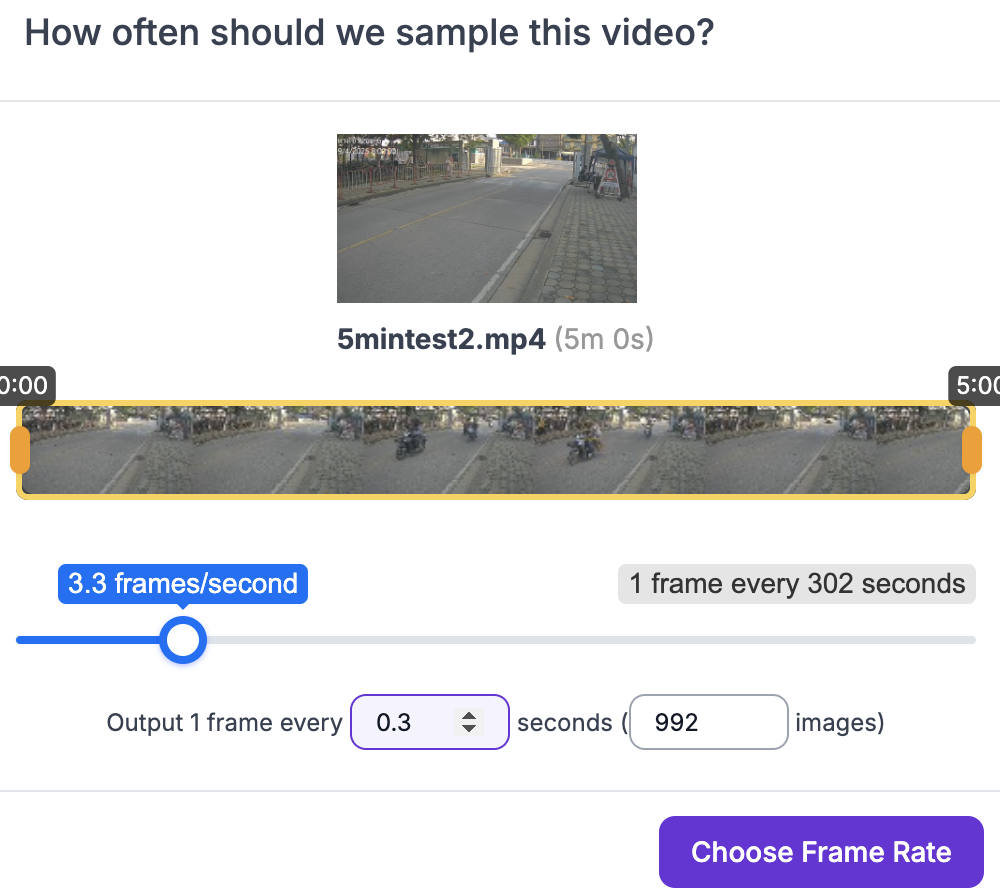
\includegraphics[width=0.5\textwidth]{Frameex.png}
		
		\vspace{0.5em}
		\textbf{Figure 3.3: Frame Extraction Image}
	\end{center}
	
	\item\textbf{Annotation:} Within Roboflow, bounding boxes were manually drawn around the target to create accurate ground truth data for supervised learning. In this project context, head and helmets are used to differentiate between a person with  a helmet on and a person without  a helmet on. Annotations were carefully reviewed to ensure consistency, especially in challenging cases such as partial occlusions or non-standard helmet designs. The figure 3.4 show an example how we draw the bounding boxes for the classes. The bounding boxes allow to make an area of detection to be easily differentiate between different classes. Therefore, the bounding box, which has to be drawn manually require to draw closely to the objects, which in this case is the head of the riders. Therefore, the differentiation between heads without helmet can be distinct from the head with helmet with minimal background. To ensure optimal detection performance, we recommend drawing bounding boxes as tightly as possible around the objects. This guideline is particularly important for researchers or practitioners who intend to follow a similar training approach or replicate our methodology.
	\begin{center}
		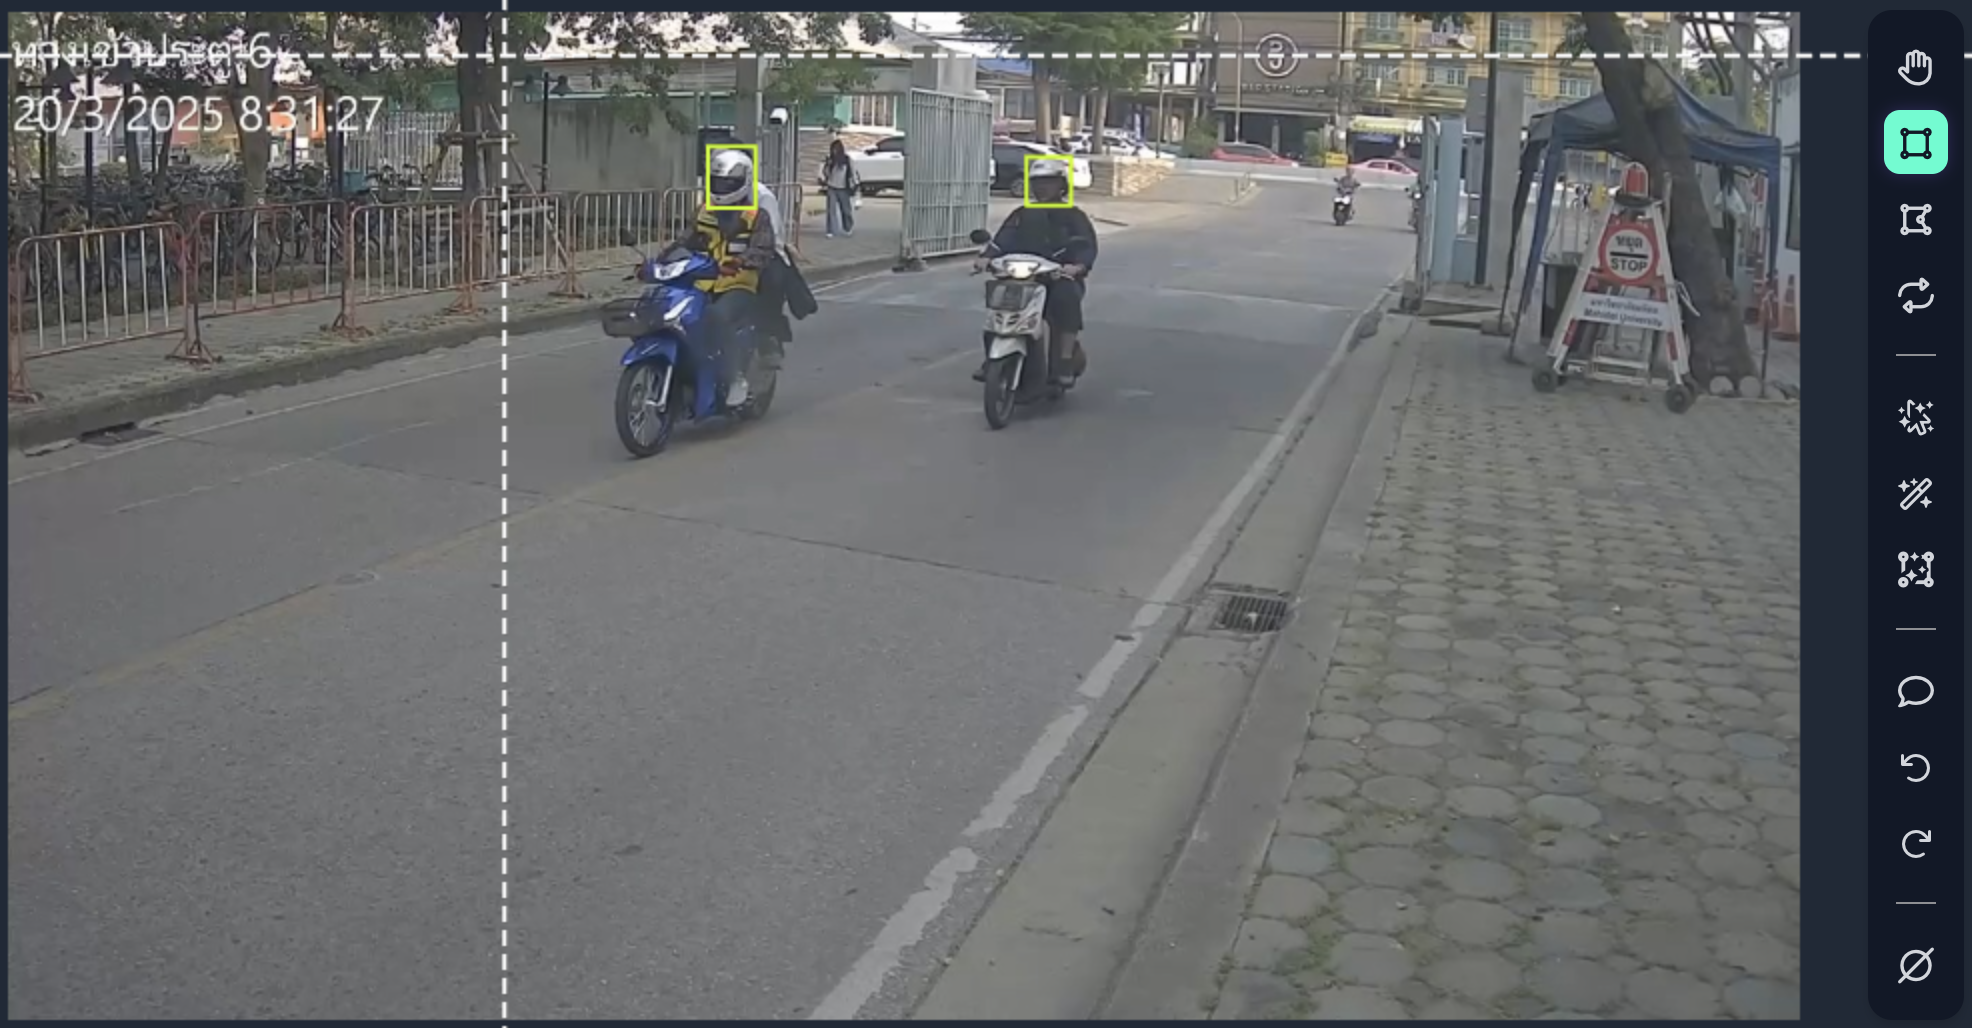
\includegraphics[width=0.8\textwidth]{Anotate.png}
		
		\vspace{0.5em}
		\textbf{Figure 3.4: Annotation Image}
	\end{center}
	\newpage
	\item \textbf{Dataset Splitting:}  The annotated dataset was divided into three subsets shown in figure 3.5: training, validation, and testing, following a common 70\%–20\%–10\% split. This allocation was selected to ensure a sufficient volume of data for effective model training, while also preserving dedicated sets for model evaluation and tuning. Specifically, 70\% of the data was used for training, providing the model with enough examples to learn relevant patterns and features from the annotated objects. The validation set, comprising 20\% of the data, played a critical role in monitoring the model's performance during training and guiding hyperparameter tuning to mitigate overfitting. Overfitting occurs when a model learns the training data too well, resulting in poor generalization to unseen data. The remaining 10\% of the data was reserved as a test set, which serves as an unbiased benchmark to evaluate the final model's performance. This partitioning strategy is widely adopted in machine learning workflows as it offers a balanced and effective framework for training, validating, and testing models. The dataset split was performed following the completion of the annotation process.
	\begin{center}
		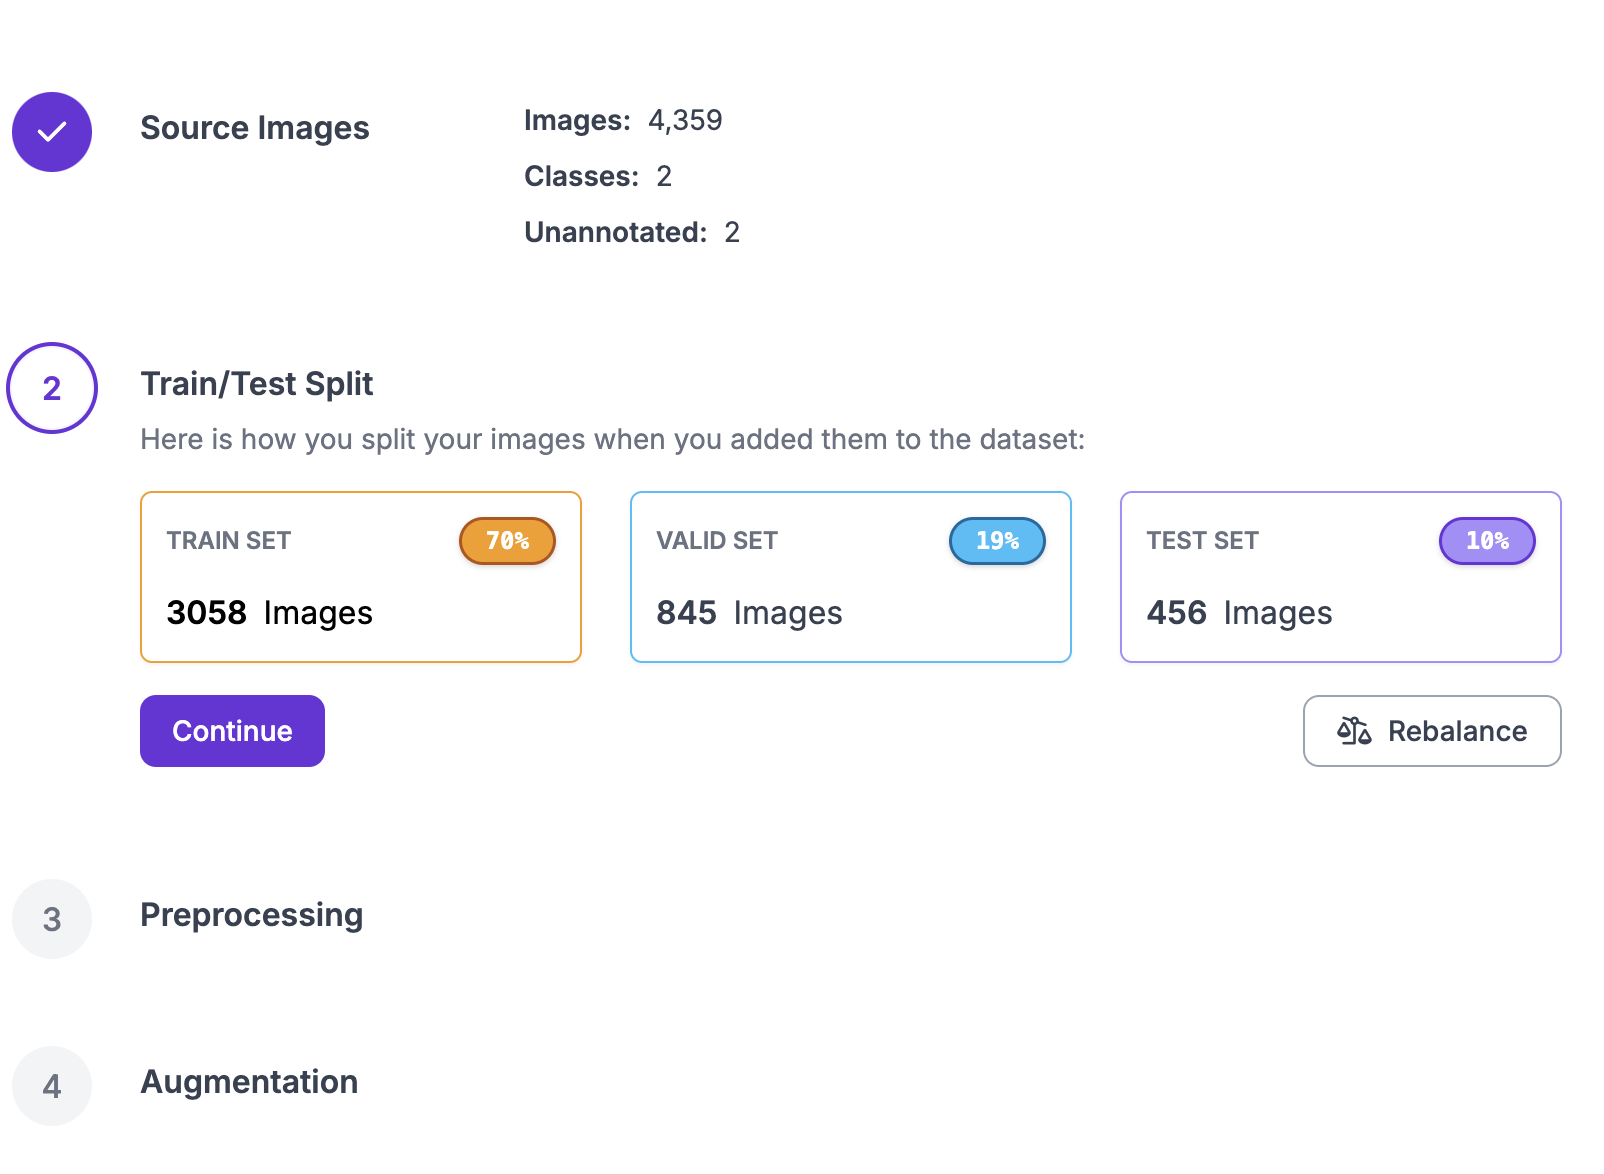
\includegraphics[width=0.8\textwidth]{Split.png}
		
		\vspace{0.5em}
		\textbf{Figure 3.5: Spliting Datasets Image}
	\end{center}
	\noindent\hspace{2.5em}Figure 3.6 illustrates the data augmentation techniques used during the model training process. These augmentations are divided into two categories: image-level augmentations and bounding box-level augmentations.
	
	
	\noindent\hspace{2.5em}The image-level augmentations applied include horizontal flipping, rotation, grayscale conversion, and exposure adjustment. These transformations alter the appearance of the entire image, thereby increasing the model’s robustness to variations in lighting, contrast, orientation, and color. Such augmentations simulate real-world environmental changes, helping the model generalize better across diverse scenes captured by CCTV footage.
	
	
	\noindent\hspace{2.5em}Bounding box-level augmentations, although not all applied in this study due to premium feature restrictions (as indicated by the “Upgrade” tags), would typically involve transformations such as crop, rotate, and shear applied directly to annotated objects. These operations preserve the alignment between bounding boxes and their corresponding objects, making them highly valuable in maintaining annotation integrity during geometric changes.
	
	
	\noindent\hspace{2.5em}In this project, specific augmentations such as horizontal flip, contrast enhancement, and brightness variation were implemented to improve detection performance under fluctuating lighting conditions and camera perspectives. These augmentations contributed to building a more resilient model capable of operating accurately across diverse visual inputs encountered in real-world traffic monitoring scenarios.
	\begin{center}
		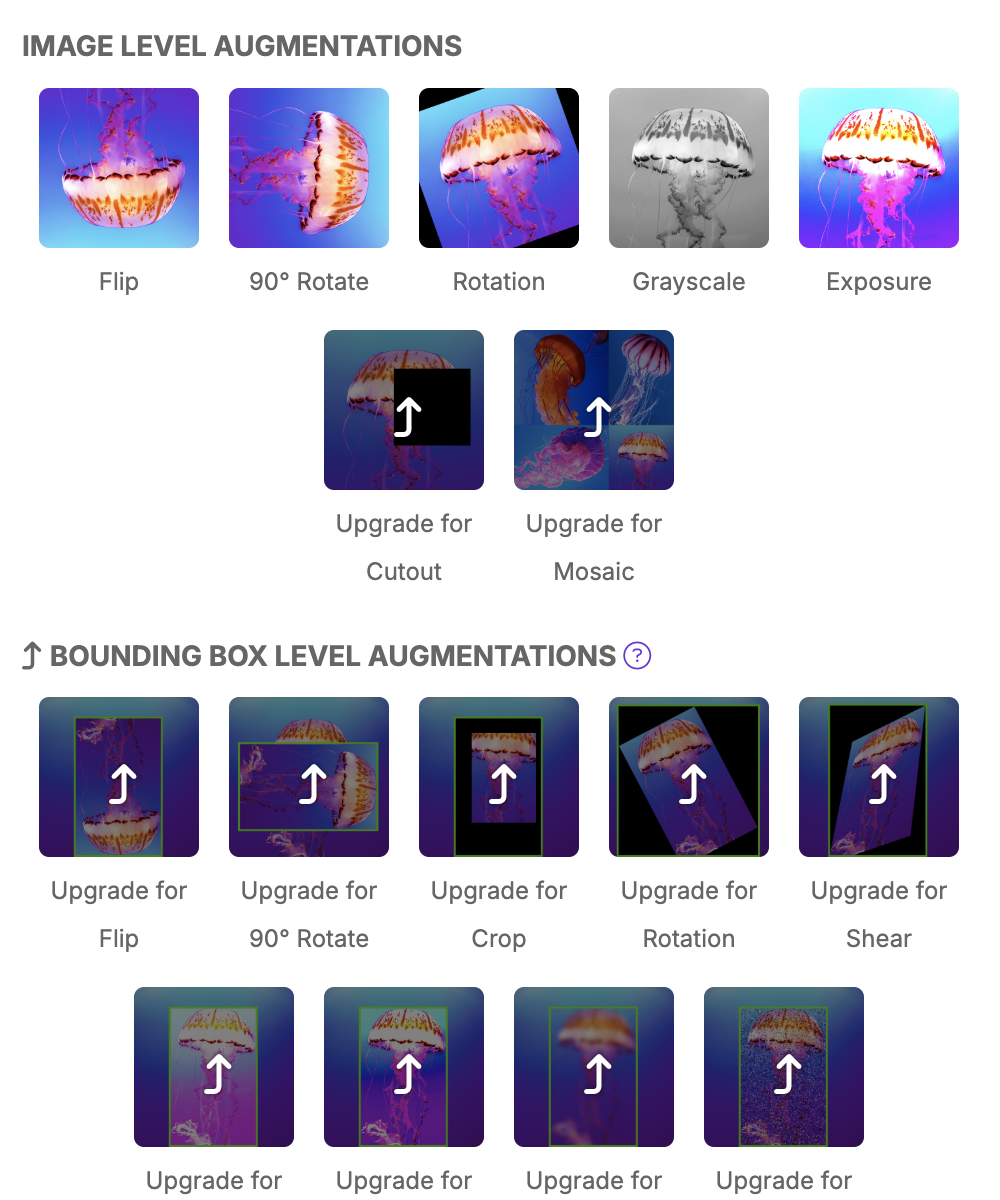
\includegraphics[width=0.8\textwidth]{Augmentation.png}
		
		\vspace{0.5em}
		\textbf{Figure 3.6: Augmentation Image}
	\end{center}
	
	\item \textbf{Data Configuration and Training:} The dataset used in this project consisted of 4,359 annotated images, divided into training, validation, and testing sets at a ratio of 70\%, 20\%, and 10\%, respectively. This split ensures a balanced distribution of data across the learning, tuning, and evaluation phases, supporting both model generalization and performance assessment.
	
	A data.yaml file was configured to organize the dataset structure and define training parameters. This configuration file specifies the relative paths to each data split, the number of object classes, and the corresponding class names used in the detection task. It acts as the main reference for the YOLOv8 framework to interpret dataset composition during training.
	
	Once the dataset and configuration were defined, the training process was initiated using the YOLOv8 framework. The training pipeline was guided by key hyperparameters—such as epoch count, image size, batch size, and learning rate—which were carefully chosen to match the dataset characteristics and available computational resources. These settings were not only critical to detection accuracy but also influenced the efficiency and stability of the model training process. Detailed descriptions and justifications of these hyperparameters are provided in the Hyperparameter Configuration section of this report.
	
	Upon completion of training, the model outputs a .pt file, which contains the learned weights, model architecture, and training metadata. This file represents the finalized version of the trained YOLOv8 model and can be used for real-time inference or integrated into post-processing tasks such as counting and visualization pipelines.
	\begin{center}
		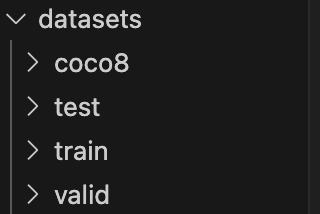
\includegraphics[width=0.8\textwidth]{Files.png}
		
		\vspace{0.5em}
		\textbf{Figure 3.7:  Files from downloaded Dataset }
	\end{center}
	\begin{center}
		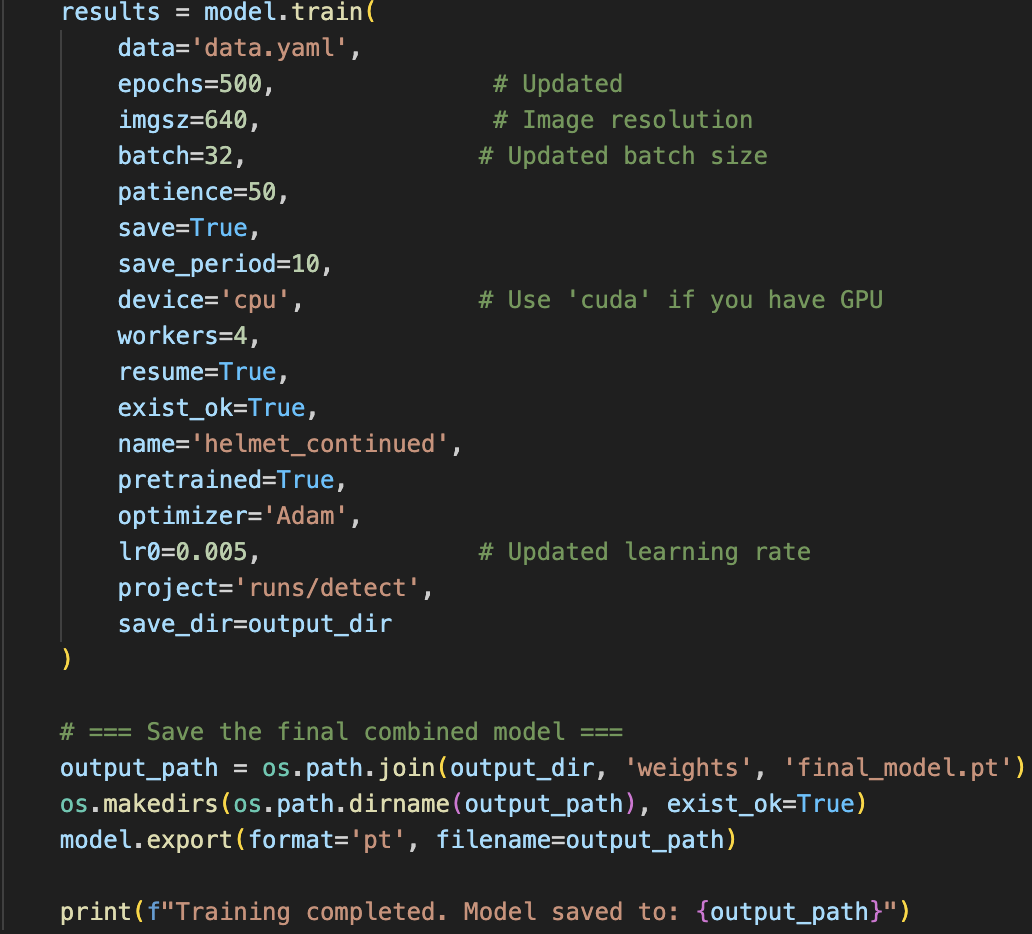
\includegraphics[width=0.8\textwidth]{yaml.png}
		
		\vspace{0.5em}
		\textbf{Figure 3.8:  Data.yaml file in VS}
	\end{center}
\end{itemize}

\section{\textbf{Counting System}}
\subsection{Helmet and Head}

\noindent\hspace{2.5em}After customizing our YOLOv8 model, which is called best\_17, by training with the dataset we have collected from CCTV footages, we implemented a counting system to track the number of helmets and unhelmeted heads by using double line counting method, while  persons and motorcycles used Bot\_Sort tracker to detected in the video.


\noindent\hspace{2.5em}For helmet and head counting, we applied a double-line counting method. This defines a "counting zone" using two vertical lines, and only counts detections whose bounding box centers fall within the zone. To prevent duplicate counting across frames, we used a rolling memory of the last ten frames. If a new detection is within a set distance (e.g., 30 pixels) of a previously counted object of the same type, it is ignored.
\newline
This method improves reliability by reducing overcounting and stabilizing results, especially for slow-moving or flickering detections. The final counts are updated in real time and displayed on the video, offering a clear summary of helmet usage and safety compliance.
\begin{figure}[H] % Optional: [H] requires \usepackage{float}
	\centering
	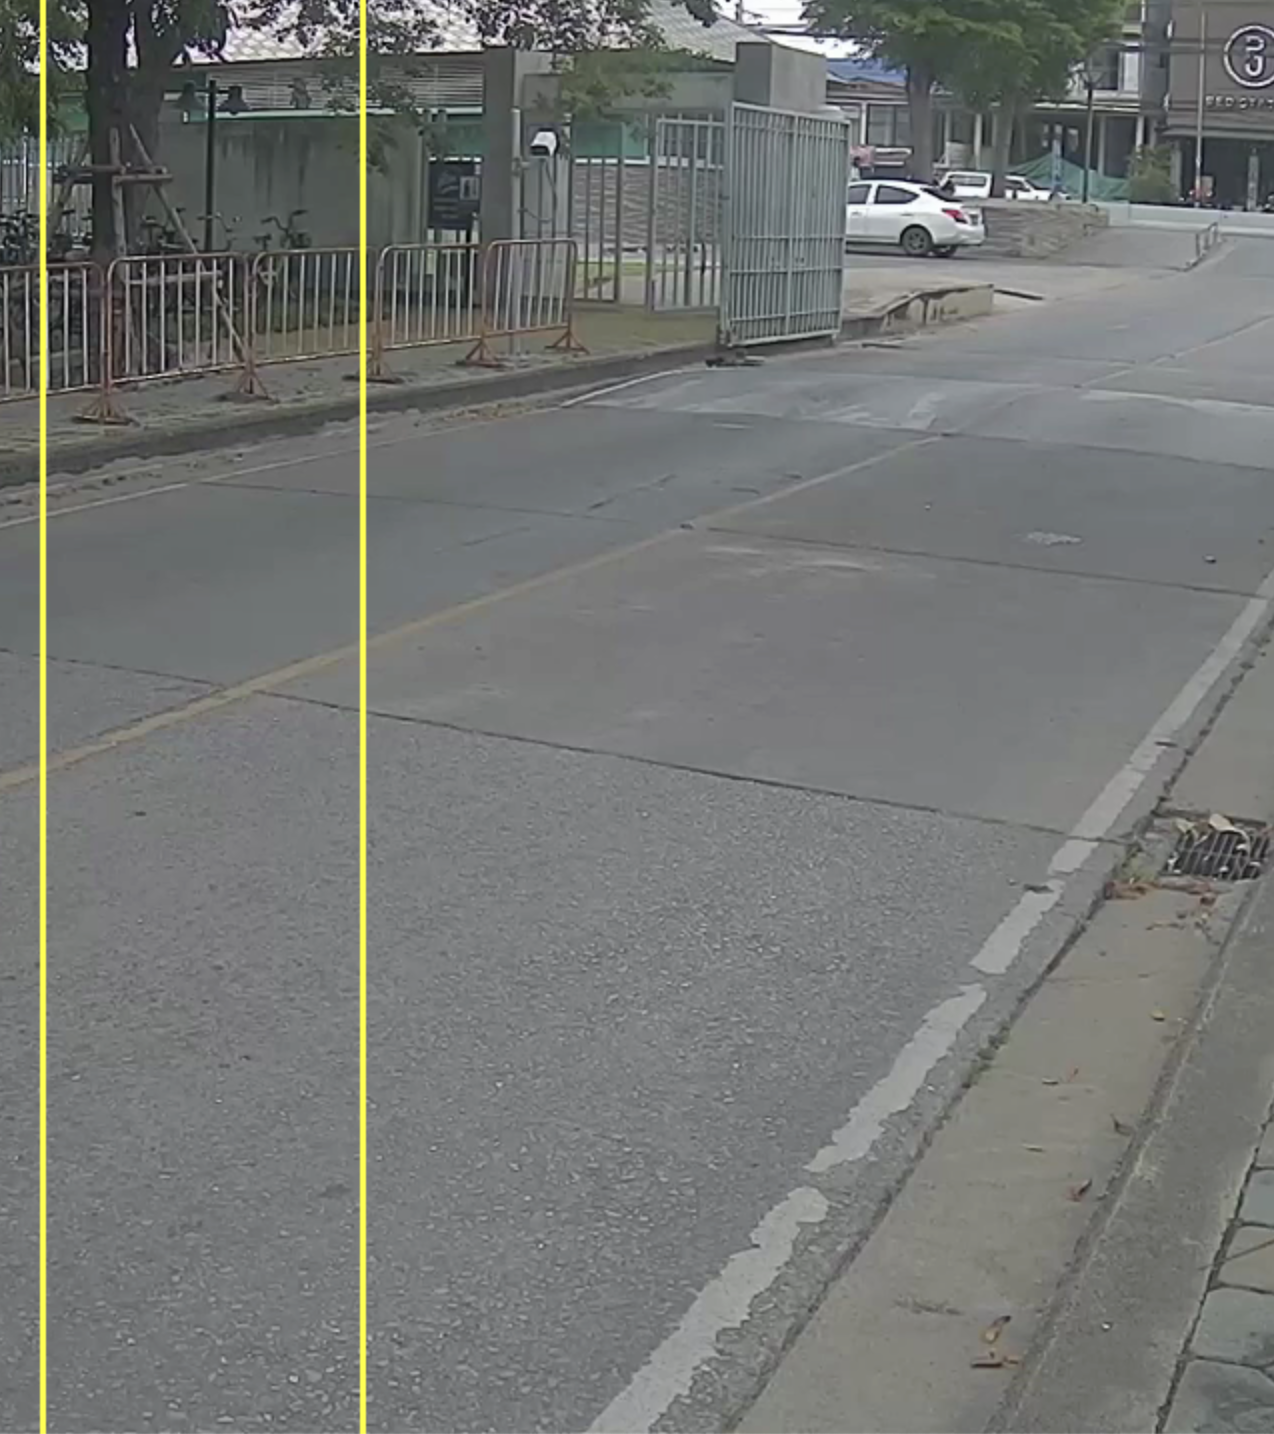
\includegraphics[width=0.5\textwidth]{headhel1.png}
	\vspace{0.5em}
	\caption*{\textbf{Figure 3.9}}
\end{figure}
\hfill
% Right side: Figure 3.3

\noindent\hspace{2.5em}Figure 3.9 illustrates the designated counting zone used for helmet and head detection. The image shows two vertical yellow lines placed 150 pixels apart, which define the area for double-line counting. When an object passes through both lines in sequence, it is registered as a valid count. This method helps reduce duplication or false counts caused by temporary detection overlaps or brief tracking loss.

\begin{figure}[H] % Optional: [H] requires \usepackage{float}
	\centering
	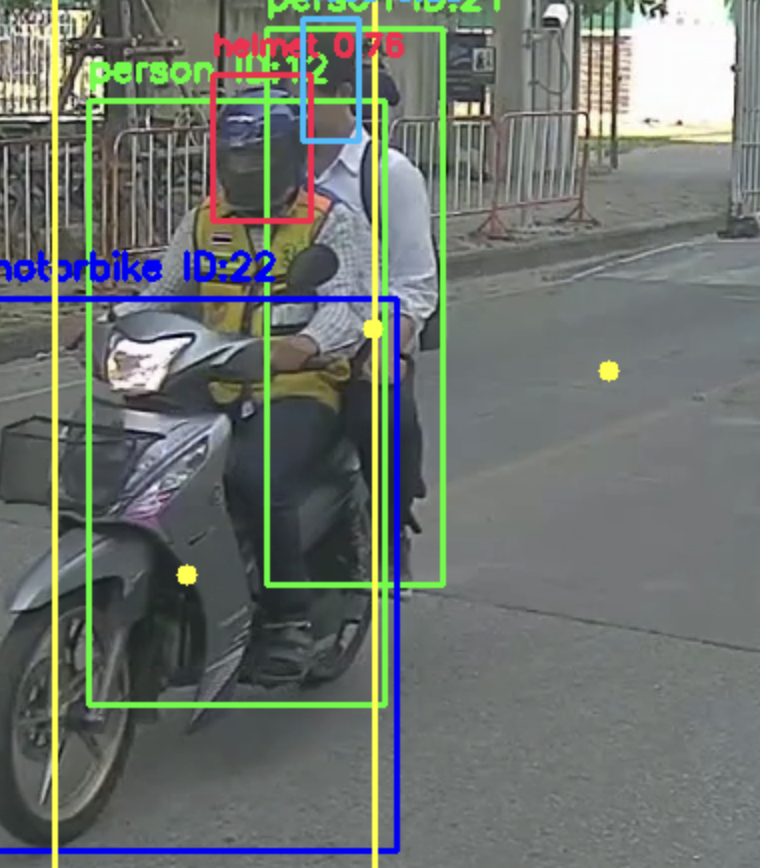
\includegraphics[width=0.5\textwidth]{headhel2.png}
	\vspace{0.5em}
	\caption*{\textbf{Figure 3.10}}
\end{figure}

\noindent\hspace{2.5em}Figure 3.10 shows an example of the double line counting system in action when objects, such as a helmet and/or a head, enter the counting zone. As seen in the image, the objects are detected and labeled with text and different colors while passing through the two vertical lines, triggering the counting logic. Two yellow vertical lines are the double counting line which are the region to only count head and/or helmet passing by. Green are the bounding box color of person, dark blue are bounding box color of motorcycle. Red are the bounding box of helmet and light blue are the bounding box of head(non-helmet). This illustrates how the system identifies and differentiates helmeted and non-helmeted riders within the defined zone.

\begin{figure}[H] % Optional: [H] requires \usepackage{float}
	\centering
	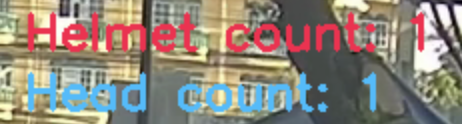
\includegraphics[width=0.5\textwidth]{headhel3.png}
	\vspace{0.5em}
	\caption*{\textbf{Figure 3.11}}
\end{figure}

\noindent\hspace{2.5em}Figure 3.11 displays the result of the helmet and head counting process, shown at the top-right corner of the screen. These values are updated in real-time after the system detects and counts objects passing through the counting zone. This visual feedback confirms the detection and classification outcome for each rider, distinguishing between helmeted and non-helmeted individuals.




\subsection{Person and Motorbike}
\noindent\hspace{2.5em}However as for the Person, and Motorbike detection we can use the Yolov8s.pt model, class 0(person), and class 3(motorbike), as their model are well polished for tracking. For the tracking use Bot-sort tracker, obtain through Roboflow ultralytics/trackers/bot\_sort.py. The tracker will be use to create specific id number for each class that has been detected. Using these id we will create center point of each classes which will be important in the counting method.


\noindent\hspace{2.5em}For the counting method, we can create a region of interest, through using open CV. From there we create a condition, to store the track id with track history. track\_history = {}   function will store the position cx, cy of the tracked object. We will use this value to identify its current and previous position to ensure that when object inside the Region of Interest, position compare is is greater than the current position objected will not be used to count, while if the current position of the tracked id compared to stored id is less than it, it can be counted inside the ROI. This is to ensure that the person, and motorbike can be counted by by what it can be tracked. The detection should look similiar to figure1.

\begin{center}
	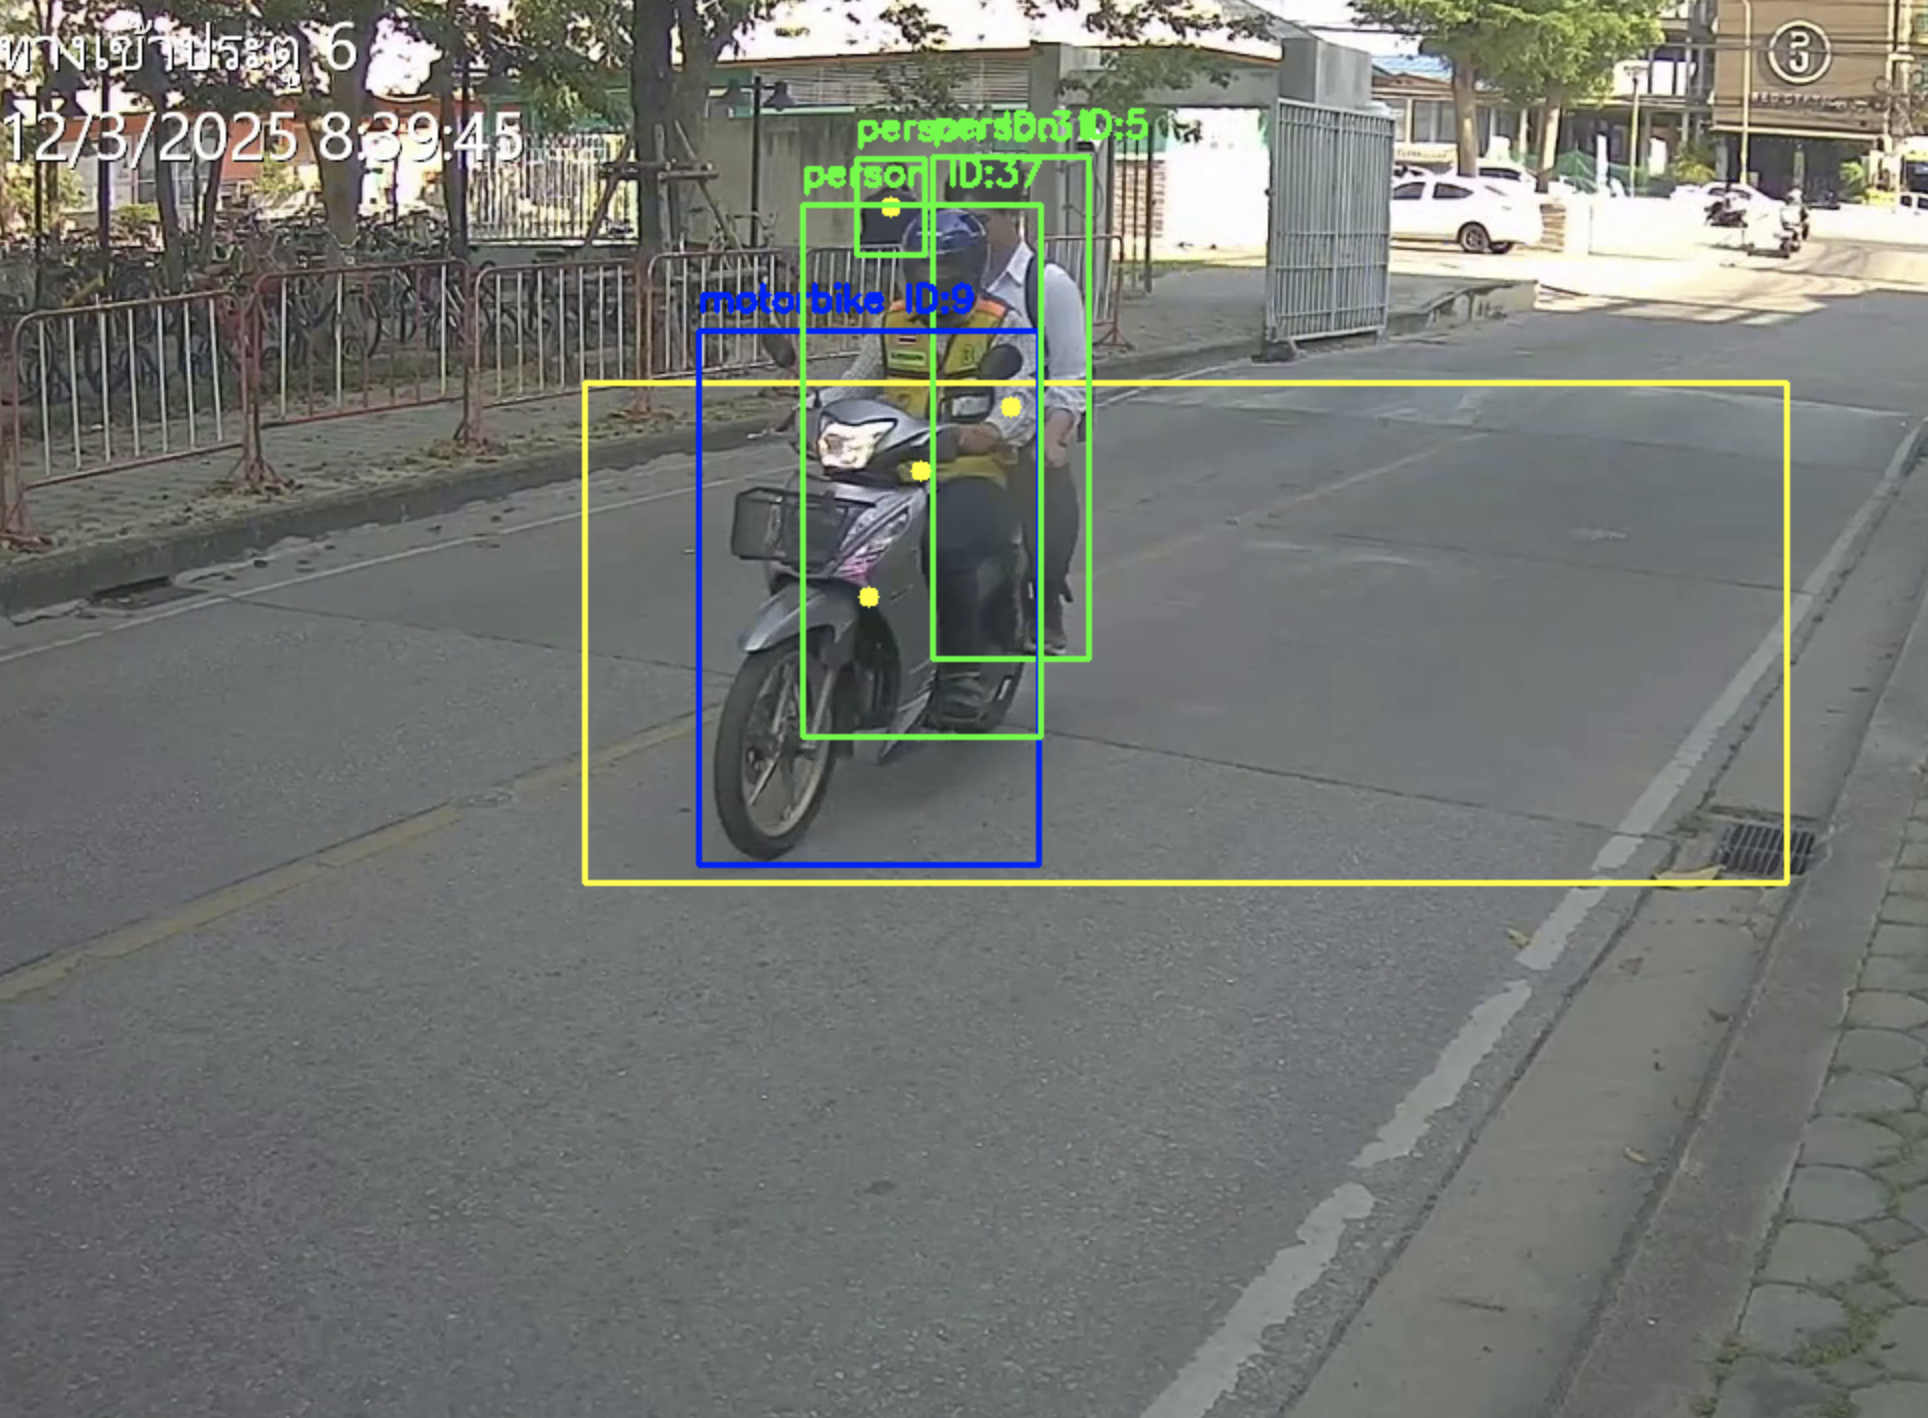
\includegraphics[width=0.5\textwidth]{fig1.png}
	
	\vspace{0.5em}
	\textbf{Figure 3.5}
\end{center}


\subsection{Output Generation}
\noindent\hspace{2.5em}The output generation phase transforms the detection and counting results into a visual and interpretable format. For each processed video frame, the system overlays bounding boxes and labels indicating the object class (helmet, head, person, or motorcycle), along with live counts displayed on the top-left corner using OpenCV. These real-time visual indicators allow users to monitor helmet usage compliance at a glance. Additionally, the system can produce an annotated video file as output, which includes all detections and updated counts across the entire duration. This output is valuable for both immediate observation and later review or reporting, providing a clear and documented summary of safety compliance in the monitored area. The images below shows the output of the system which after we run the program, will show live dection of the video input, and the save video file after the program completed the detection, we save it as a way to easier analyse and observe the detection through video playback, as analysing it live while running maybe not be as efficient.
\begin{center}
	\begin{minipage}{0.45\textwidth}
		\centering
		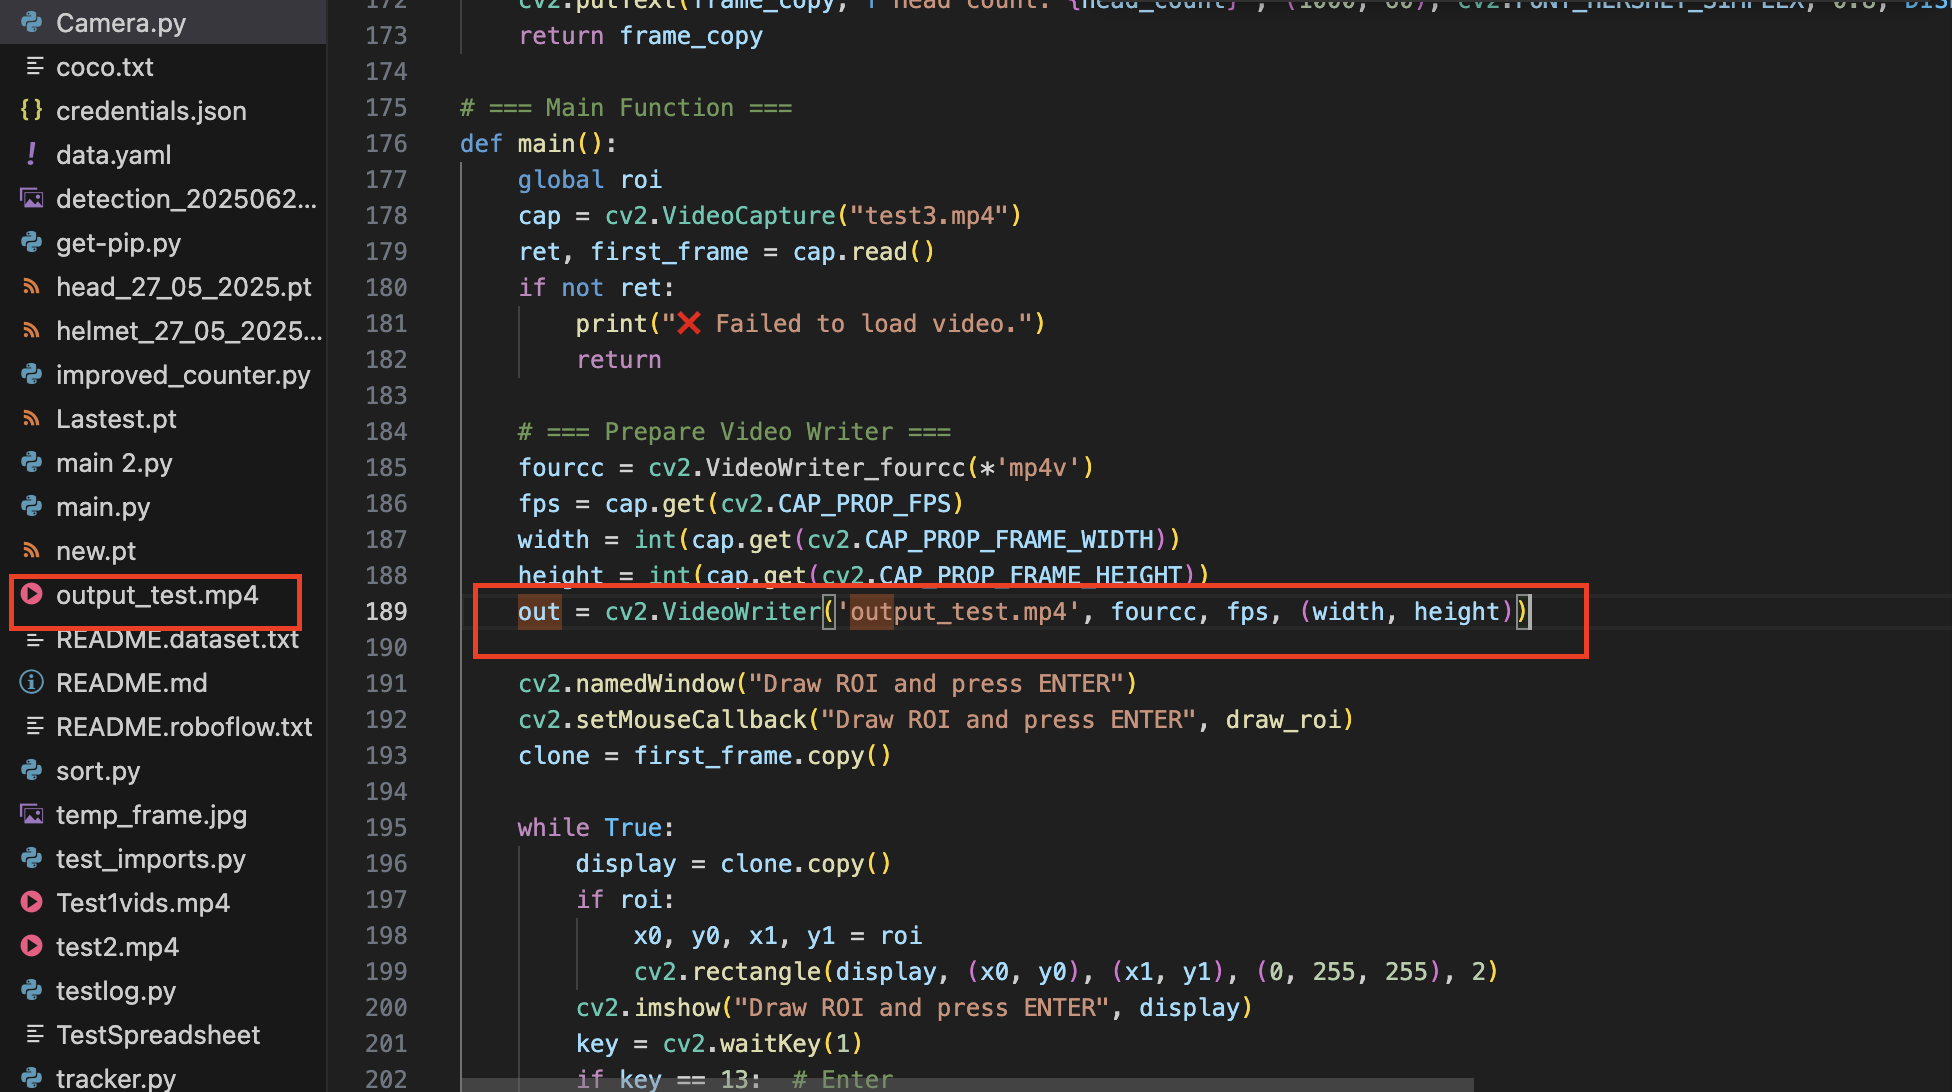
\includegraphics[width=\linewidth]{out.png}
		\vspace{0.7em}
		
		\textbf{Figure 3.4.1: Saved output Video}
	\end{minipage}
	\hfill
	\begin{minipage}{0.45\textwidth}
		\centering
		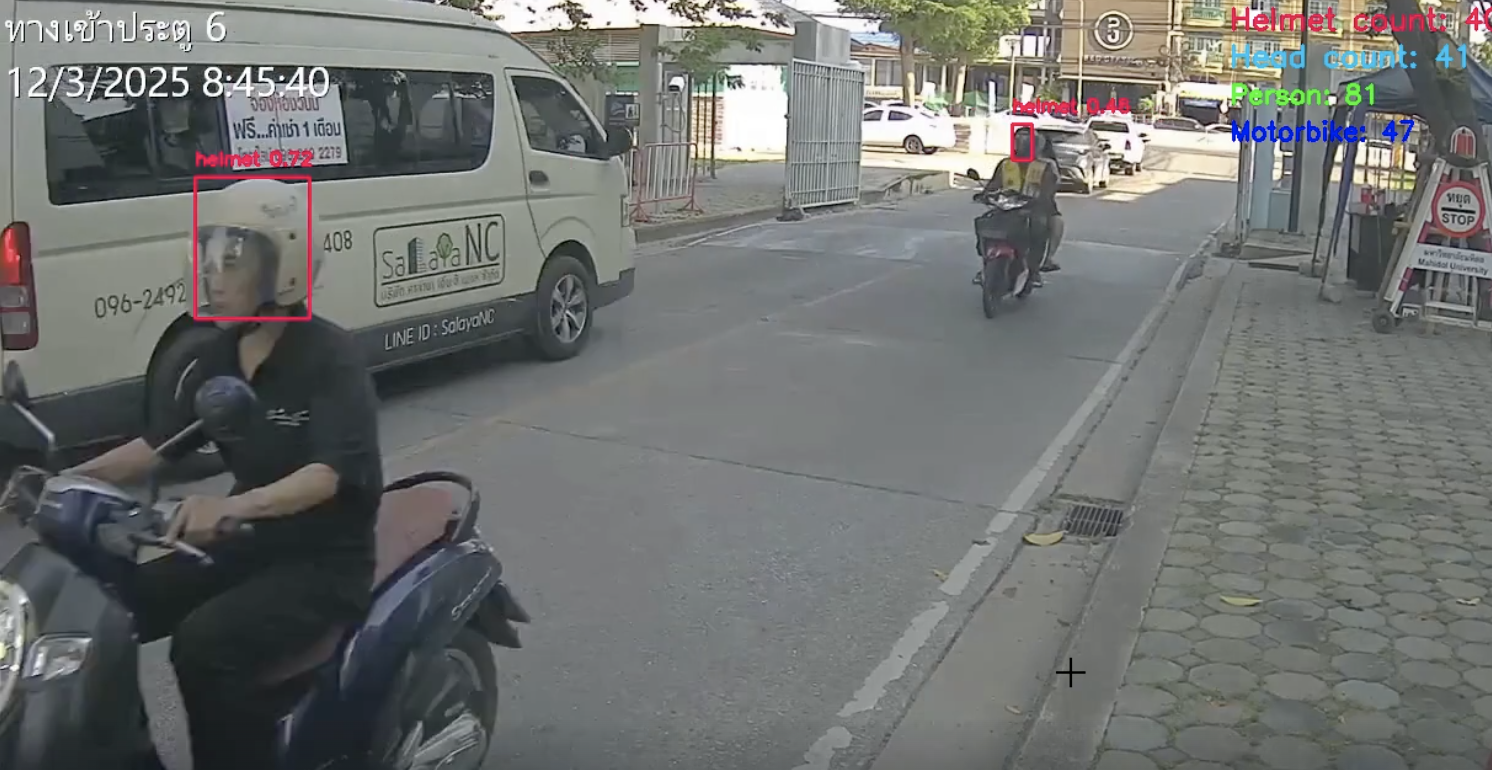
\includegraphics[width=\linewidth]{live.png}
		\vspace{0.5em}
		
		\textbf{Figure 3.4.2: Live Output Generation}
	\end{minipage}
\end{center}


\subsection{Storing Output in Google Sheet API}
\noindent\hspace{2.5em}After the output has been generated, we store the detection into a log using Google API from the video steam. The Google API integration is used for logging and evidence storage for helmet violation cases. Firstly as mention the two model, YOLOv8 pre-trained model, and custom model for head/helmet detection. How the system is works is, when a head is detected within the zone. The frames will be stored, using cv2 to snap-shot the specific frame of head detection. We log the detections events to Google Sheet, it records, the timestamp, head detection, alert, and link to Google Drive file to the captured image.


\noindent\hspace{2.5em}The credentials.json file can be obtained through Google API, the system will connect to pre-defined Google Sheet as we name them(Data log) and appneds the new rows with each detection events that occurs, the image are uploaded to Google Drive using the Drive API, and public access links are generated per log. This implementation allows users to store datas of the detection, this is to allow scalable and automated solution for monitoring helmet violations. The result is as seen in the figure below.

\begin{center}
	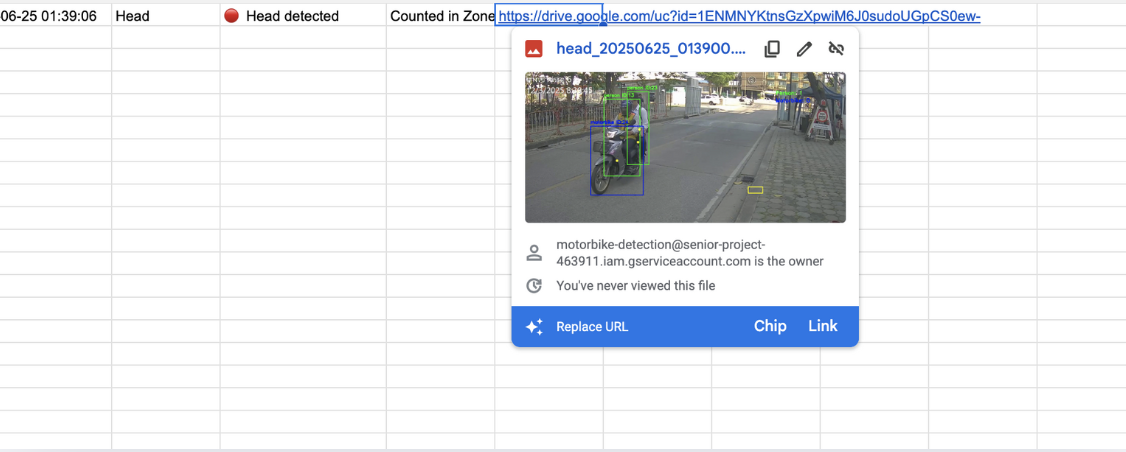
\includegraphics[width=1\textwidth]{api.png}
	
	\vspace{0.5em}
	\textbf{Figure 3.6}
\end{center}

\section{Tools and Frameworks}
\begin{itemize}
	\item \textbf{YOLOv8 Framework}: For object detection.
	\item \textbf{Libraries}: Python libraries such as ultralytics, opencv-python, numpy, collections.
	\item \textbf{Annotation Tools}: Roboflow.
	
\end{itemize}


\section{Hyperparameter Configurations}
During the training process, serveral key herparameters were manually selected to balace the performce, the model accuracy and accordingly to our local computation resrouces.

\textbf{Epochs} = 500, this is to ensure suffieicent exposeure to the training datasets. It will allow the model to learn patterns, and improve generalization overtime. However we can stop the early depending on our resources and depending on overfitting.

\textbf{Image Size} imgsz = 640 (image resolution) 640x640 pixel is most commonly use parameter. This will also help decrease the traning time. However for smaller objects like head and helmet detection. Training them on 640x640 is enough, however in some circumstances when training very far, helmet and head that are annotated are risk to losing fine-grained details. This is important as it is very essential for detecting small overlapping objects. For our case we annotate them after they pass the bumper, we have checked that at this area before hand that when resolution was 640x640, it was not too grainy for traing. The image belows shows the annotated image that was resized to 640x640 for training. 


\begin{center}
	\begin{minipage}{0.45\textwidth}
		\centering
		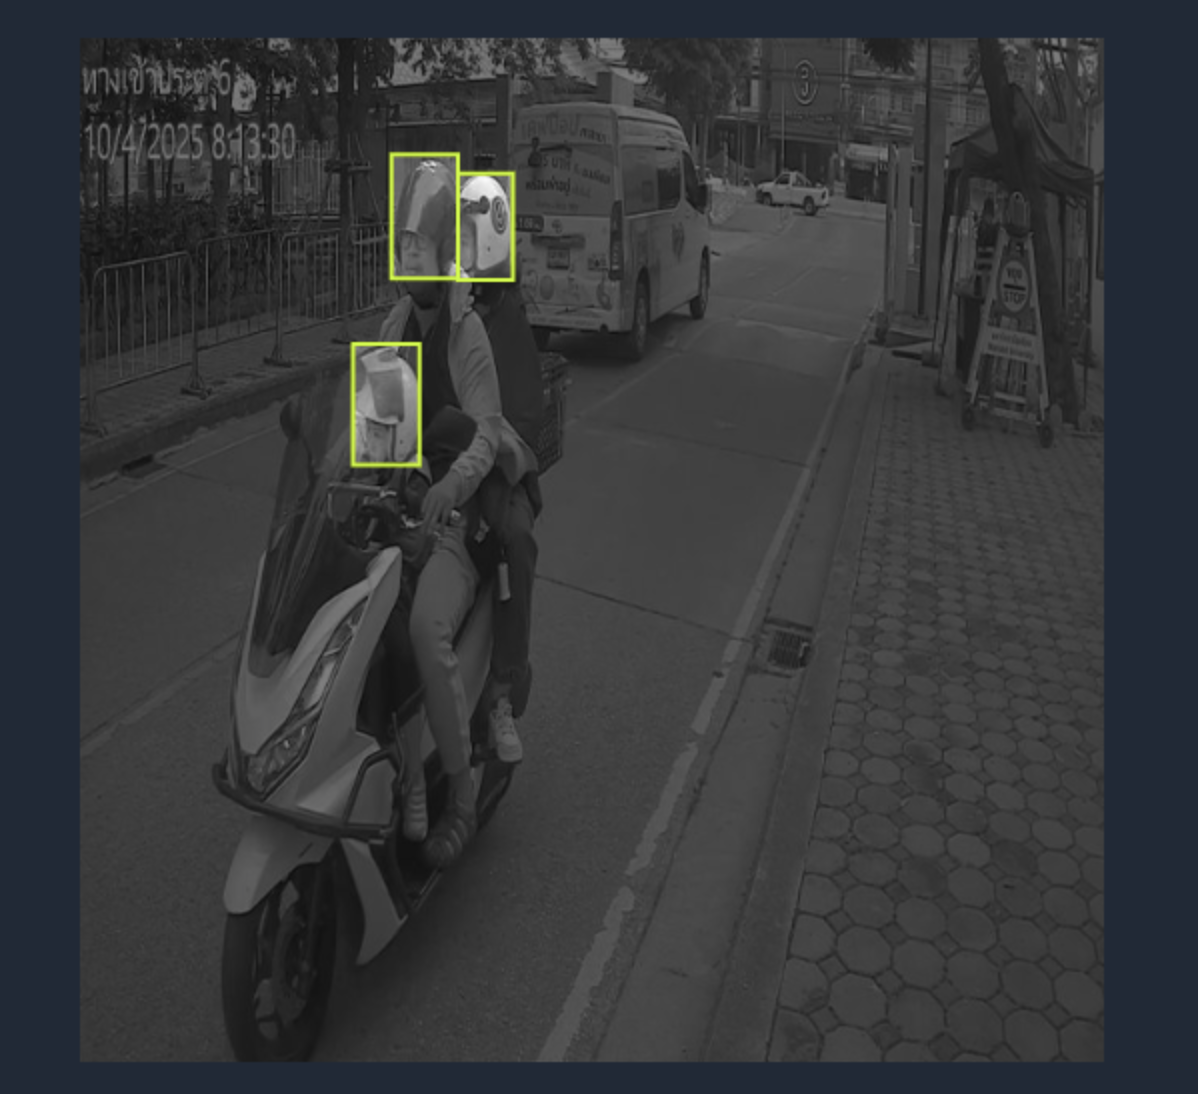
\includegraphics[width=\linewidth]{ano1.png}
		\vspace{0.7em}
		
		\textbf{Figure 3.6.1: Resized Image }
	\end{minipage}
	\hfill
	\begin{minipage}{0.45\textwidth}
		\centering
		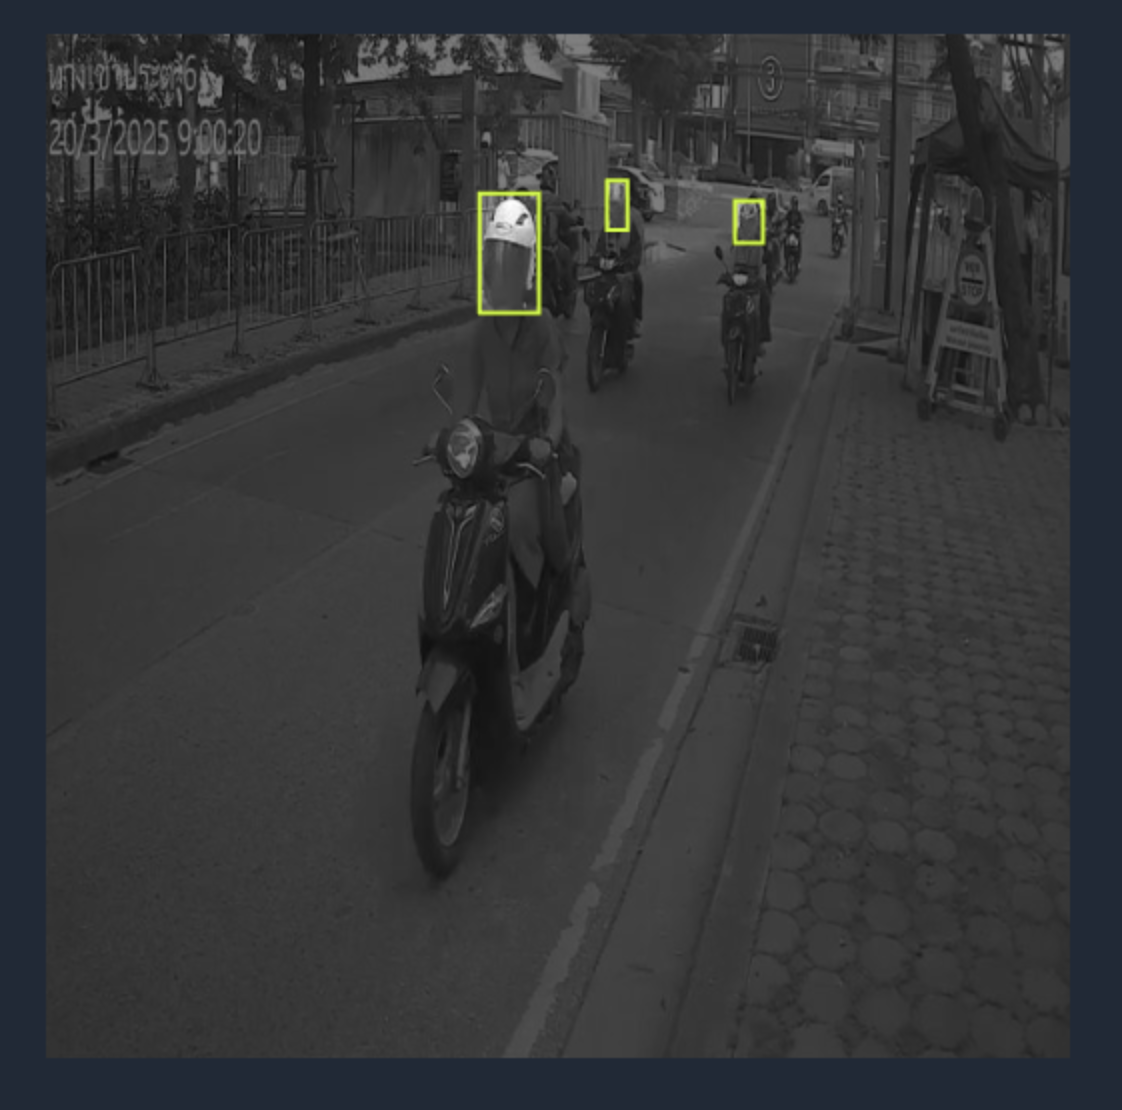
\includegraphics[width=\linewidth]{ano2.png}
		\vspace{0.5em}
		
		\textbf{Figure 3.6.2: Resized Image }
	\end{minipage}
\end{center}




\textbf{Batch Size} =32, this is due to primarily contrained by the GPU, as larger batches can lead larger samples, and faster convergency. Nonetheless, batch size 32istill alowws for reasonable effieicnt traning and consistent model updates. This value can be changed depending on the GPU memory. While a larger batch size could have potentially accelerated training and stabilized gradient updates, our hardware limitations required a compromise at 32 images per batch.

\textbf{Learning Rate} = 0.005. Setting it to this value helps to cacilitate steady learning without causing instability. If it was too high, it could result in model to overshoot the optimal solution during traning. This value is also recommended by YOLOv8.



\section{Performace Evaluation}

\noindent\hspace{2.5em}The trained YOLOv8 models were evaluated using standard object detection metrics: \textbf{mean Average Precision (mAP)}, \textbf{precision}, and \textbf{recall}. These metrics provide a quantitative assessment of detection accuracy and were used to track the progression and performance of each model iteration. The primary metric, \textbf{mAP}, measures the area under the precision-recall curve and is defined as:

\[
\text{mAP} = \frac{1}{N} \sum_{i=1}^{N} \text{AP}_i
\]

where $\text{AP}_i$ represents the Average Precision for class $i$, and $N$ is the total number of classes. mAP offers a comprehensive evaluation by considering both false positives and false negatives, making it a reliable indicator of overall model accuracy.

\textbf{Precision}, defined as

\[
\text{Precision} = \frac{\text{True Positives}}{\text{True Positives} + \text{False Positives}},
\]

measures the proportion of correctly predicted positive detections among all predicted positives. High precision indicates that most detections are correct, which is crucial for reducing false alarms in safety-critical applications like helmet detection.

\textbf{Recall}, defined as

\[
\text{Recall} = \frac{\text{True Positives}}{\text{True Positives} + \text{False Negatives}},
\]

reflects the model's ability to correctly identify all relevant objects in the frame. High recall ensures that few objects are missed, which is particularly important for applications where under-detection can compromise system reliability.

Together, these metrics were used to compare multiple trained models, guiding the selection of the best-performing version for downstream tasks such as accurate counting of helmets and heads in real-world traffic footage.

\begin{center}
	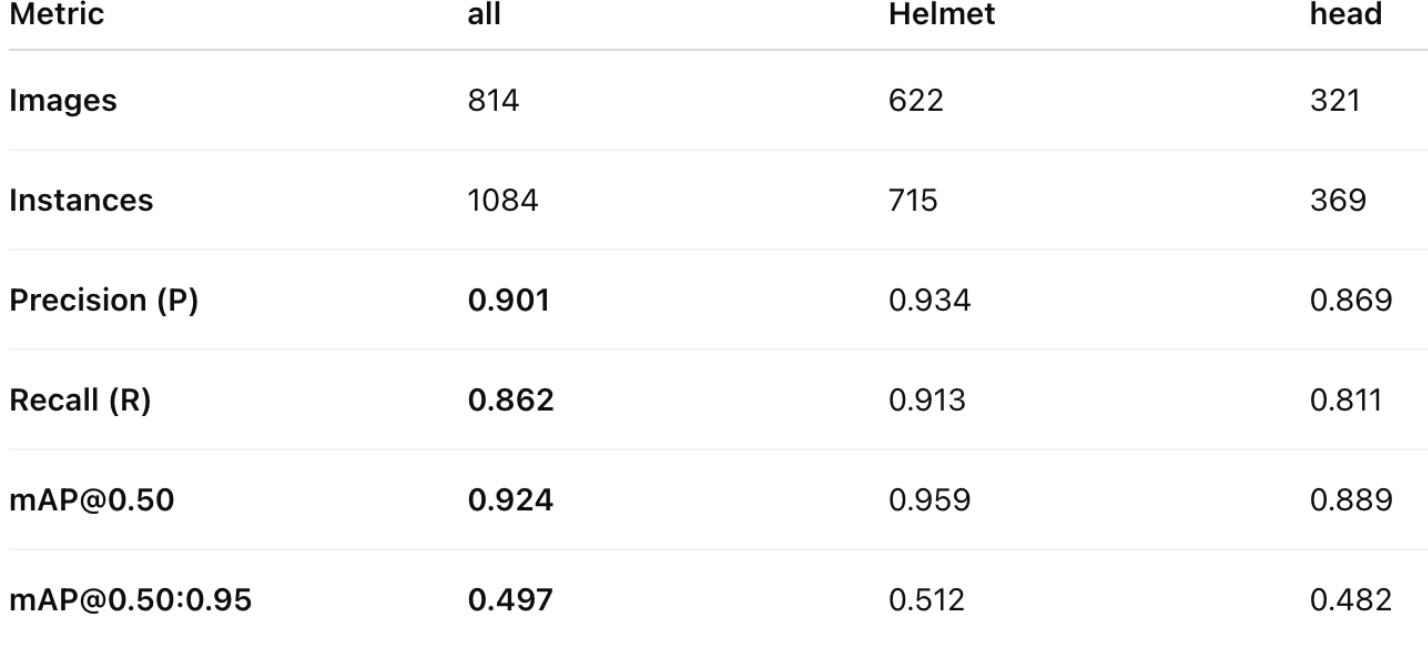
\includegraphics[width=1\textwidth]{performance.eva.png}
	
	\vspace{0.5em}
	\textbf{Figure 3.7}
\end{center}

\noindent\hspace{2.5em}The evaluation results in figure 3.7 demonstrate that the best custom YOLOv8 model performs strongly in detecting both helmet and heads(non-helmet), with particularly high accuracy in helmet detection. Overall, the model achieved a precision of 0.901 and recall of 0.862 across all classes, indicating reliable and consistent predictions. For the helemt class specifically, the model attained satisfying performance with a precision of 0.934, recall of 0.913, and a high mAP@0.50 of 0.959. This suggests that the model can effectively identify helmets with minimal false positives and false negatives. In comparison, the head class yielded slightly lower results, with a precision of 0.869, recall of 0.811, and mAP@0.50 of 0.889, reflecting more variation or complexity in detecting uncovered heads. The overall mAP@0.50:0.95 score of 0.497, while moderate, still indicates acceptable performance under stricter localization conditions. These results affirm the model’s suitability for real-time helmet usage monitoring, particularly in scenarios where accurate helmet detection is critical.

\begin{center}
	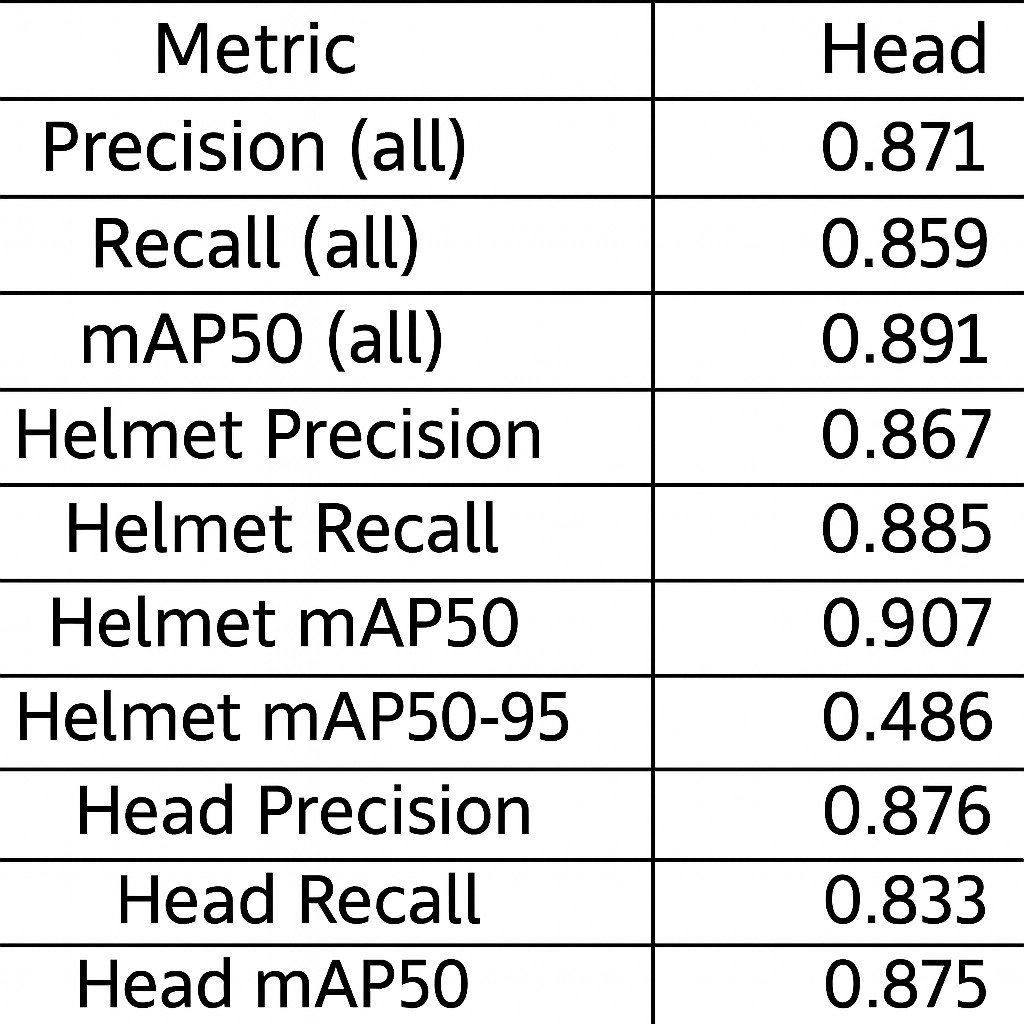
\includegraphics[width=1\textwidth]{performance.eva2.png}
	
	\vspace{0.5em}
	\textbf{Figure 3.8}
\end{center}
\noindent\hspace{2.5em}Figure 3.8 shows the previous model performace evaluation, which is call Head\_model. In comparing the performance of the updated helmet and head detection model, which is figure 3.7, to the previous version, several improvements are evident. 

\noindent\hspace{2.5em}The current model achieves an overall precision of 0.901 and recall of 0.862, both higher than the previous model’s precision of 0.871 and recall of 0.859, suggesting better accuracy and detection coverage. Helmet detection has particularly improved, with the current model reaching a helmet precision of 0.934, recall of 0.913, and mAP@0.50 of 0.959, outperforming the previous model’s respective values of 0.867, 0.885, and 0.907. Head detection has also seen slight gains, with the current model achieving 0.869 precision, 0.811 recall, and 0.889 mAP@0.50, compared to 0.876, 0.833, and 0.875 in the earlier version. Additionally, the current model maintains a solid mAP@0.50:0.95 of 0.497 overall, indicating better localization performance under stricter IoU thresholds. These enhancements reflect a more robust and reliable detection system, making the current model better suited for real-world deployment in helmet compliance monitoring scenarios.